\documentclass[tikz, margin=0.1pt]{standalone}
\usepackage{tikz} 

\begin{document}

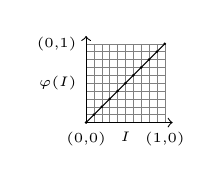
\begin{tikzpicture}[scale=1, dot/.style = {circle, fill, minimum size=#1, inner sep=0pt, outer sep=0pt}, dot/.default = 1pt] 

% Grid
\draw[step=0.1cm,gray,very thin] (0,0) grid (1,1);  % Decrease step to add more gridlines

% Axes
\draw[thin,->] (0,0) -- (1.1,0) node[anchor=north] at (0.5, 0) {\tiny $I$};
\draw[thin,->] (0,0) -- (0,1.1) node[anchor=east] at (0,0.5) {\tiny $\varphi(I)$};

% Points on axes and labels
\node[anchor=north] at (0,0) {\tiny (0,0)};
\node[anchor=east] at (0,1) {\tiny (0,1)};
\node[anchor=north] at (1,0) {\tiny (1,0)};

% Dots and lines
\node[dot] at (0,0) {};
\node[dot] at (.1,.1) {};
\node[dot] at (.2,.2) {};
\node[dot] at (.3,.3) {};
\node[dot] at (.4,.4) {};
\node[dot] at (.5,.5) {};
\node[dot] at (.6,.6) {};
\node[dot] at (.7,.7) {};
\node[dot] at (.8,.8) {};
\node[dot] at (.9,.9) {};
\node[dot] at (1,1) {};
\draw[thin] (0,0) -- (0.1, 0.1) -- (0.2, 0.2) -- (0.3, 0.3) -- (0.4, 0.4) -- (0.5, 0.5) -- (0.6, 0.6) -- (0.7, 0.7) -- (0.8, 0.8) -- (0.9, 0.9) -- (1, 1);

\end{tikzpicture}

\end{document}